\documentclass[11pt,a4paper]{article}

\usepackage[utf8]{inputenc}
\usepackage{graphicx}
\usepackage{float}
\usepackage[singlespacing]{setspace}
\usepackage[left=2.5cm,right=2.5cm,top=2cm,bottom=2cm]{geometry}

\setlength{\parskip}{5pt plus 1 pt minus 1 pt}

\begin{document}

\thispagestyle{empty}
\pagestyle{empty}

{\bf\centerline{{\huge Resume}}}
\vspace{6pt}

\centerline{Adrian Regenfuß (*28.10.1997)}
\centerline{Weinschenkstraße 4a}
\centerline{80999 Munich, Germany}
\centerline{+49 89 80 92 86 94, +49 160 95 96 43 99}
\centerline{a.regenfuss@posteo.de}
\smash{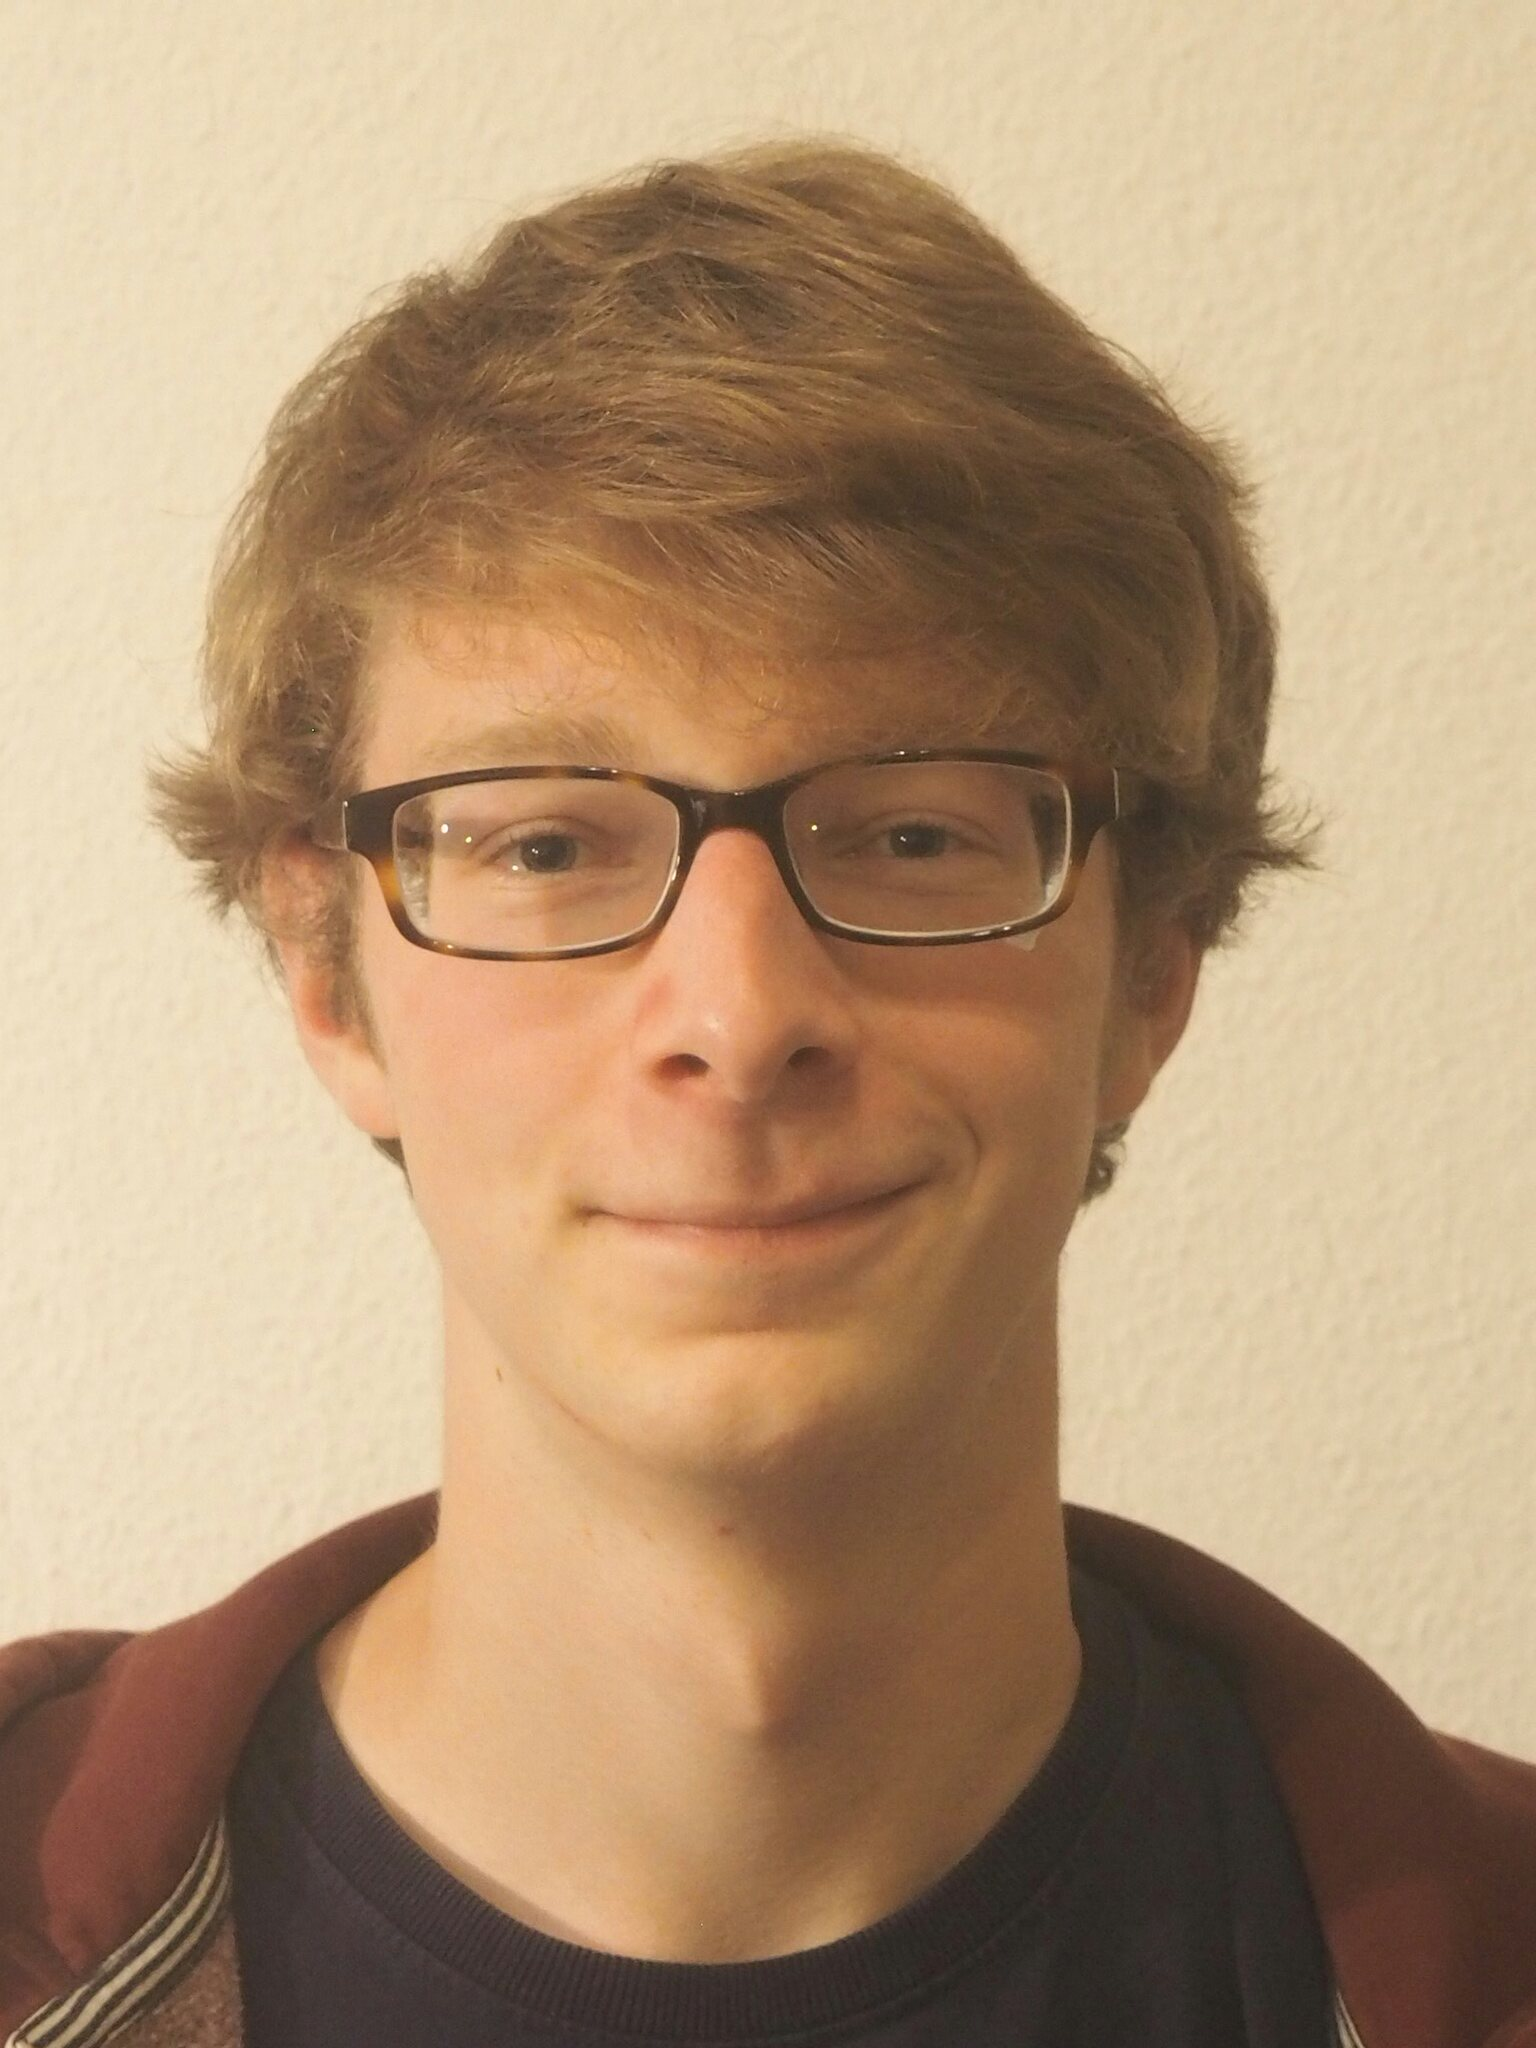
\includegraphics[scale=0.3]{./farbe.jpg}}

\vspace{5pt}

Interested and motivated student with ambition to learn
about new technologies and software. Personal experience in programming
and administrating Unix systems. Curious about professional software
design and development methods.

Finished school in summer 2016 with excellent grades. Currently doing a
Computer Science Bachelor at the TU München.

\section*{Technical skills}
\begin{itemize}
	\setlength{\itemsep}{1pt}
	\item[]{\bf Languages}: C, Java, Lua, OCaml
	\item[]{\bf Operating Systems}: Unix, Windows, Plan 9 from Bell labs
	\item[]{\bf Tools}: git, make, gdb, awk, sed, regular expressions, LaTeX
	\item[]{\bf Database}: SQL
\end{itemize}

\section*{Employment history}
\begin{itemize}
	\setlength{\itemsep}{1pt}
	\item Internship at the Deep Learning Competence Center in the German Research Center for Artificial Intelligence
	(Deutsches Forschungszentrum für Künstliche Intelligenz, www.dfki.de), with focus on analysis of
	visual data using convolutional neural networks.\\
	\hfill September - November 2016
	\item Summer job at Allocation Network GmbH in Munich (software maintenance and testing of a commercial supplier management system)

	\& eliminate duplicates in the companies exchange mail
	server database - design, build and test)
	\hfill June 2014
	\item Internship at the auction house Karl \& Faber in Munich \hfill July 2013, November 2013
\end{itemize}

\section*{Recent software projects}
\begin{itemize}
	\setlength{\itemsep}{1pt}
	\item Work on a filesystem-based distributed chat client using the tox protocol
	\item Automatic generation of a word dictionary with word
	frequencies by analyzing Wikipedia
	\item High performance stream-based generation of chains
	in formal systems (based on Douglas Hofstadter's ''MU``)
	\item Contributions to the open source projects ogg122 (github.com/dimkr/ogg122),\\
	sbase (git.suckless.org/sbase) and human (git.z3bra.org/human/log.html)
	\item More projects at github.com/pranomostro
\end{itemize}

\section*{Education}
\begin{itemize}
	\setlength{\itemsep}{1pt}
	\item[] Studying Physics at the Technical University of Munich \hfill Since September 2016
	\item[] Highschool, finished with General Certificate of Education/GCE (German Abitur).
	Final grade of 1.5 on a scale of 1 to 6, where 1 is the best mark. Karlsgymnasium Pasing, Bavaria.
	\hfill February 2012 - June 2016
	\item[] Performed a 2 week language study travel to Clermont-Ferrand, France
	\hfill June 2013, April 2014
	\item[] Completed a 1 week language study travel in Broadstairs, England \hfill July 2012
	\item[] Kaiserin Friedrich Gymnasium in Bad-Homburg, Hessen \hfill 2008 - 2012
	\item[] Peter-Härtling Schule in Friedrichsdorf, Hessen \hfill 2004 - 2008
\end{itemize}

\section*{Extracurricular activities}
\begin{itemize}
	\setlength{\itemsep}{1pt}
	\item[] Co-creation of an audio guide for a historic German labor camp near Munich
	\hfill March 2016
	\item[] Spent 1 term at Scotch College, Melbourne \hfill July - September 2014
	\item[] Completed a 2 week language study travel in Melbourne, Australia \hfill August 2013
\end{itemize}

\section*{Additional abilities}
\begin{itemize}
	\setlength{\itemsep}{1pt}
	\item Speaking and writing English fluently
	\item Reading and speaking French fluently (level B1)
	\item Touch typing with 70 words per minute
\end{itemize}

\section*{Interests}
\begin{itemize}
	\setlength{\itemsep}{1pt}
	\item Programming
	\item Open source software projects
	\item Software algorithms and machine learning
	\item Taek-Won-Do
	\item Playing Piano, Clarinet and Baritone saxophone
	\item Philosophy
\end{itemize}

\section*{References}
Andreas Vollmann, Director - Allocation Network GmbH Munich (mail@allocation.net)

\end{document}
